\documentclass{article}
\usepackage{qtree}
\usepackage{graphicx}
\usepackage[left=1.25in,right=1.25in]{geometry}
\begin{document}
\begin{enumerate}
\item \textbf{Decision Trees and ID3}
  \begin{enumerate}
  \item The result of splitting on $A$:
    \begin{center}
      \Tree [.3:4 1:2 2:2 ]
    \end{center}
    The associated remainder (weighted entropy):
    \[-\left(\frac17\ln\frac13+\frac27\ln\frac23+\frac27\ln\frac24+\frac27\ln\frac24\right)\approx.669\]

    And for splitting on $B$:
    \begin{center}
      \Tree [.3:4 2:3 1:1 ]
    \end{center}
    \[-\left(\frac27\ln\frac25+\frac37\ln\frac35+\frac17\ln\frac12+\frac17\ln\frac12\right)\approx.679\]

    So splitting on $A$ provides a result with a slightly lower
    remainder, and hence slightly higher information gain.

    Splitting on $A$ may be preferable because the entropy, i.e.
    information required after the split, is lower.  Intuitively,
    splitting on $A$ might be more useful because it provides a more
    even separation of the data into the true and false branches, and
    hence a shorter tree; splitting on $B$ might also be useful
    because if $B$ is true, then that branch is completely decided.

    This shows that ID3 has inductive bias for shorter (more balanced)
    trees.
  \item 
    In the following tree, going down a left branch left indicates
    True, and right indicates False.

    \Tree [ .A [.B F [.C F T ] ] [ .B T T ] ]
     
    In the first stage, splitting on A generates the lowest remainder.
    Then considering the other three attributes. Attributes B and C
    are tied for lowest remainder for both values of A; we split on B
    in both cases.
    
    If A is True and B is True, there is only one case, in which the
    classification is False. Otherwise, there are two cases that are
    exactly dependent on C.

    If A is False and B is True, there is one case, in which the
    classification is True. Otherwise, there are two cases that cannot
    be separated, in which case we arbitrarily pick True.
 
    6 of 7 are correctly identified by the tree. 

  \item Consider the following tree, that also correctly identifies 6
    out of 7.  Again, going left indicates True, and going right
    indicates False.

    \Tree [ .B [ .C T F ] [ .C F T ] ]

    We see that although the ID3 algorithm is designed to greedily try
    to get the shortest / simplest tree by maximizing information gain
    at every split, it does not always end up choosing the shortest or
    simplest tree, probably due to the myopic nature of the greedy
    algorithm.
 
  \end{enumerate}
\item \textbf{ID3 with Pruning}
  \begin{enumerate}
    \setcounter{enumii}2
  \item Since the pruned version does slightly better than the
    unpruned on 10-fold cross-validation, there is probably some
    overfitting: reducing complexity improves perfomrance.
    (Specifically, clean unpruned had success rate 0.87; clean pruned
    0.89, noisy unpruned 0.78, noisy pruned 0.80.)

    However, it is interesting to note this difference (by about the
    same amount) for both clean and noisy data, which indicates that
    generalization to noisier data is not affected by pruning, which
    indicates that ID3 is not overfitting to training data noise.
    %TODO: verify???
  \item  
    \begin{enumerate}
    \item Our implementation uses instance weight throughout. It is
      implemented already to calculate entropy of a split, find the
      majority label in a branch, evaluate correct / incorrect, and so
      on. Then it uses this information ***

      If decisions were made only based on instance counts, there
      would be no change between rounds of boosting, so nothing new
      would happen and all the classifiers would be essentially the
      same. The performance of AdaBoost is based on the idea that
      later classifiers pay more attention to the instances that
      earlier ones have missed, so as to make up for their mistakes.

%      However, when we're not boosting it just weights things evenly. 
 
%%       AdaBoost on ID3 would not work if splitting decisions were made
%%       by counting instances instead of summing weights, because
%%       AdaBoost is based on the idea that you update weights based on
%%       which data instances need better fitting.
    \item In that case, the total weight of true and false instances
      are both .5, so the entropy is 1:
      \[-\left(\frac12\log_2\frac12+\frac12\log_2\frac12\right)=1\]

%%       Weighted entropy of $\{x_1,\ldots,x_n\}$ where $y_1=T$, $y_i=F$
%%       else, $w_1=0.5$, and other weights are $0.5/(n-1)$: by
%%       definition $entropy(D)=-\sum_{y\in Y} \frac{W_y}{W} \log_2
%%       \frac{W_y}{W}$ and $W_y=\sum_i w_k(i) I(y_i=y)$; we have
%%       $W_{T}=0.5$, $W_{F}=0.5(n-1)^{-1}(n-1)=0.5$, $W=1$, and
%%       so $$entropy(D)=-\left[ \frac{1}{2}\log_2\frac{1}{2} +
%%         \frac{1}{2}\log_2\frac{1}{2} \right] = 1$$
    \end{enumerate}
    \begin{enumerate}
    \item Boosting seems to do noticeably better on the other methods
      for clean data, but not on noisy data (see figure).

      \begin{center}
        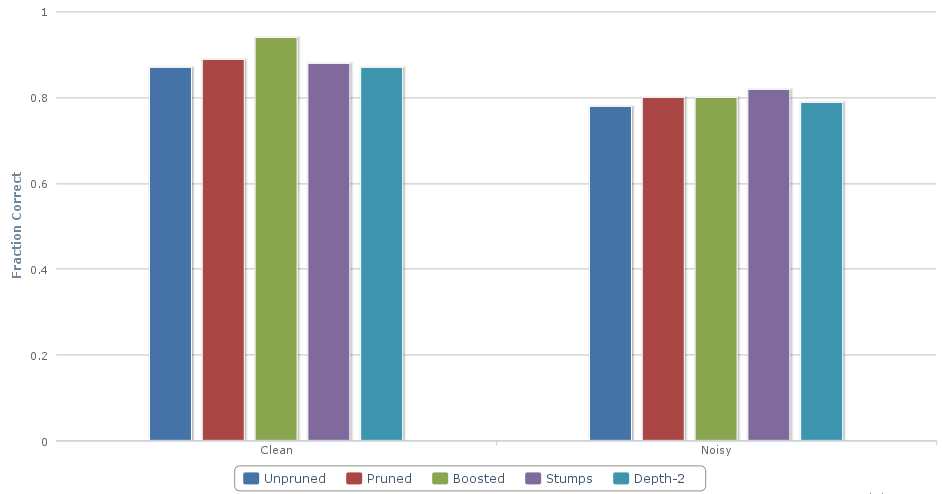
\includegraphics[scale=.4]{graph.png}
      \end{center}

      The drop that boosting suffers due to noisy data is much larger
      than the drop that pruned trees suffer, indicating that boosting
      is badly particularly affected by noisy data. Perhaps this means
      that boosting is bad for inconsistent data; maybe the
      inconsistent elements, since some of them will always be wrong,
      tend to end up with very large weights, taking attention away
      from the majority of the data.

%%       ******TODO:WARNING:CAVEAT*****Why does boosting do so poorly??
%%       on task compare boosting parameters***** Boosting appears to
%%       work consistently better than the other methods on noisy data.
%%       In particular, this appears to indicate that boosting may be
%%       less sensitive to overfitting by increasing the preference
%%       bias. ****???****
 
    \item Based on the figure above, we see that stumps do slightly
      better than depth-2 trees, which looks like overfitting.
    \item If we did not know that boosting produces a maximum-margin
      classifier, we would be surprised that boosting depth 1 on 10
      rounds is improved upon by boosting depth 1 on 30 rounds on
      clean data. Perhaps we'd think that performance would taper off
      before that many rounds of boosting. However, the fact that it
      is margin-maximizing indicates that it should improve, so that
      it continues to approach the decision boundary. On the other
      hand, there is no improvement for the analogous tests on noisy
      data, which we can attempt to explain by the fact that with
      added noise, the decision boundary is less well-defined, so that
      further approaching the decision boundary is no longer fruitful.
      It is additionally surprising why this is not true for depth 2,
      which we can only attempt to explain as in part 2dii.

      On the other hand, it might be surprising that the performance
      hardly increases despite the many more rounds of
      boosting. Perhaps the maximum-margin nature of AdaBoost means
      that it reaches peak performance very quickly.
    \item More rounds of boosting training generally increases
      accuracy in cross-validated test sets. It appears that sometimes
      an extra iteration of training decreases accuracy a bit, but the
      trend is overall positive until the plateau, although the
      variation in accuracy can be pretty large (i.e., boosting 4
      times is the same as boosting 10 times, though the peaks in
      between go up).
    \end{enumerate}
  \end{enumerate}
\item Consider the unpruned tree generated by ID3 from the BCW data:
  {\small
\begin{verbatim}
attr = 4
    1 False
    2 False
    3 attr = 9
         1 False
         2 False
         3 True
         5 False
         8 True
    4 attr = 6
         2 True
         3 True
         4 False
    5 True
    6 attr = 2
         5 True
         7 True
         8 False
    7 True
    8 True
    9 True
   10 True
\end{verbatim}
}

  {\tt False} and {\tt True} represent leaves with those labels; {\tt
    attr = n} indicates an internal node that splits on attribute
  number $n$ (according to the numbering in the data file); its
  children are listed immediately after it. The number before any of
  those indicates the attribute value of the parent node that leads to
  that node.

  From this, it looks like attribute 4 (uniformity of cell shape) is
  the most important attribute in determining malignancy. In fact, it
  looks like malignancy is more likely with higher attribute values:
  the two lowest values branch straight to {\tt False} leaves, while
  the four highest go to {\tt True}. Meanwhile, the first child node
  has two {\tt False} leaves and three {\tt True} ones, while the
  other two  Indeed, looking over the original
  data set gives the following statistics:

  \begin{center}
    \begin{tabular}{|c|c|c|}\hline
      malignant? & attribute value & frequency \\\hline
      1 & 0 & 42 \\\hline
      2 & 0 & 5 \\\hline
      3 & 0 & 5 \\
      3 & 1 & 2 \\\hline
      4 & 0 & 2 \\
      4 & 1 & 4 \\\hline
      5 & 1 & 8 \\\hline
      6 & 0 & 1 \\
      6 & 1 & 4 \\\hline
      7 & 1 & 5 \\\hline
      8 & 1 & 7 \\\hline
      9 & 1 & 1 \\\hline
      10 & 1 & 14 \\\hline
    \end{tabular}
  \end{center}

  It can be clearly seen that there is quite a good correlation; a
  stump that split on this one attribute would achieve 95\% accuracy.

  The three children nodes split on the attributes normal nucleoli,
  single epithelial cell size, and clump thickness.
\end{enumerate}
\end{document}
